\section{Continuità di massa}\label{sec:continuità-massa}
L'equazione di \emph{continuità di massa} descrive come la massa interiore della stella varia con il raggio. Si può scrivere nella seguente maniera:
\begin{equation}\label{eq:continuità-massa}
    \dfrac{\ud M(r)}{\ud r} = 4 \pi r^2 \rho(r)
\end{equation}

\begin{figure}
\centering
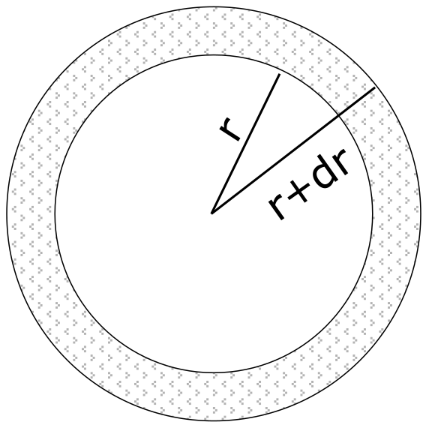
\includegraphics[width=0.25\textwidth]{immagini/continuita-massa.png}
\caption{Guscio sferico infinitesimo a distanza $r$ dal centro. All'interno del guscio, a causa della simmetria sferica, ipotizziamo che la densità e la temperatura siano costanti.}
\label{fig:continuità-massa}
\end{figure}

Per ricavarla consideriamo un guscio sferico infinitesimo di stella, come in figura~\ref{fig:continuità-massa}. Siccome all'interno di tale guscio la densità di ogni elemento è la stessa, a causa della simmetria sferica della struttura, possiamo ricavare il valore di massa all'interno di tale guscio:
\[
    \ud M(r) = 4 \pi r^2 \rho(r) \ud r
\]
da cui segue immediatamente l'eq.~\eqref{eq:continuità-massa}. Consideriamo il caso semplice di densità costante, in cui $\rho(r) = \Bar{\rho}$, si può calcolare in  maniera semplice la massa presente entro il raggio $r$:
\[
    M(r) = \int_0^{M(r)} \ud m(r) = \int_0^r \ud r' 4 \pi {r'}^2 \rho(r') = \frac{4}{3} \pi r^3 \Bar{\rho}
\]
